\section{Lecture-01}

\textbf{Question:} what did we mean by the derivative $f'(a)$?\\
\textbf{Answer:} Let \textcolor{red}{$U$ be an open subset} of $\mathbb R$ and $f:U\rightarrow \mathbb R$ a function. Then $f$ is differentiable at $a$, with derivative $m$, if and only if
\begin{equation}
\label{diff_1}
    \lim_{h\rightarrow 0}\frac{1}{h}\left( \underbrace{f(a+h)-f(a)}_{\Delta f} - \underbrace{mh}_{(*)} \right)=0
\end{equation}
$(*):$ linear function of $\Delta x=h$.\\
\textbf{Question:} Why impose the domain $U$ that needs to be an open set?\\ 
\textbf{Answer:} Write the answer.\\
The function $mh$ that multiplies $h$ by the derivative $m$ is thus a linear function of the change in $x$. This definition emphasizes the idea that a function $f$ is differentiable at a point $a$ if the increment $\Delta f$ to the function is well approximated by a linear function of the increment $h$ to the variable, this linear function is $f'(a)h$. Let's see how we can confirm that:\\
Suppose $f(x)$ is our desired function and we want to approximate the function in the neighborhood at $x=a$. For this purpose, we will draw several straight lines through the point $(a,f(a))$ and see which line approximates the function best. Here, the best means, the linear line should approximate the function well at $x=a+h$. Suppose the slope of that linear function is $m$.   
\begin{center}
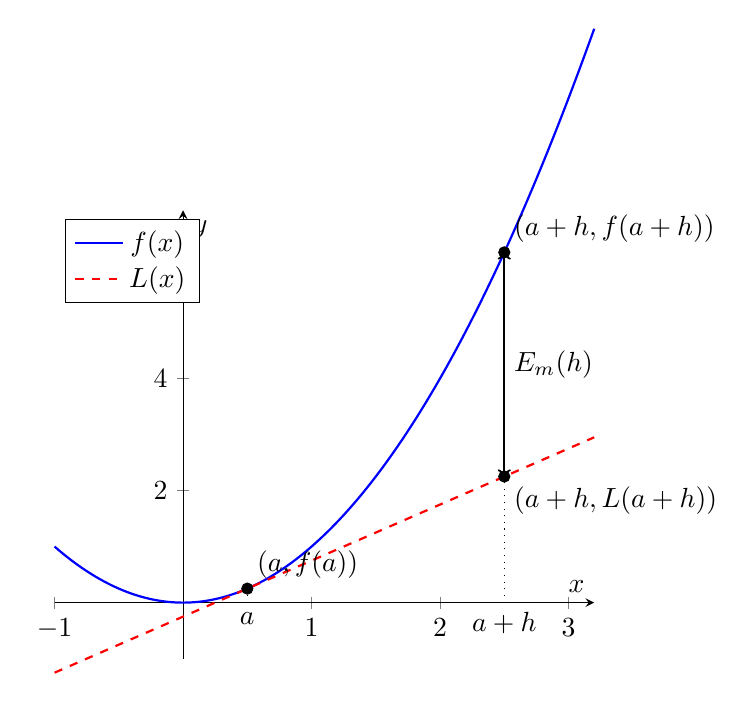
\begin{tikzpicture}
\begin{axis}[
    axis lines = middle,
    xlabel={$x$},
    ylabel={$y$},
    xmin=-1, xmax=3.2,
    ymin=-1, ymax=7,
    samples=200,
    domain=-1:3.2,
    legend style={at={(0.02,0.98)},anchor=north west},
    clip=false
]

% ---- Choose a function (example) ----
% f(x)=x^2, f'(x)=2x
\addplot[blue, thick] {x^2};
\addlegendentry{$f(x)$}

% ---- Parameters a and h ----
\def\a{0.5}
\def\h{2}

% Values at a, and at a+h
\pgfmathsetmacro{\fa}{(\a)^2}
\pgfmathsetmacro{\apH}{\a+\h}
\pgfmathsetmacro{\fapH}{(\apH)^2}

% Tangent line at x=a:  y = f(a)+f'(a)(x-a)  ;  f'(a)=2a
\addplot[red, thick, dashed] {2*\a*(x-\a)+\fa};
\addlegendentry{$L(x)$}

% Tangent prediction at x=a+h:  L(a+h)=f(a)+f'(a)h
\pgfmathsetmacro{\LapH}{\fa + 2*\a*\h}

% ---- Mark key points ----
\addplot[black, mark=*] coordinates {(\a,\fa)};
\node[above right] at (axis cs:\a,\fa) {$(a,f(a))$};

\addplot[black, mark=*] coordinates {(\apH,\fapH)};
\node[above right] at (axis cs:\apH,\fapH) {$(a+h,f(a+h))$};

\addplot[black, mark=*] coordinates {(\apH,\LapH)};
\node[below right] at (axis cs:\apH,\LapH) {$(a+h,L(a+h))$};

% Vertical reference lines at a and a+h
\addplot[dotted] coordinates {(\a,0) (\a,\fa)};
\node[below] at (axis cs:\a,0) {$a$};

\addplot[dotted] coordinates {(\apH,0) (\apH,\fapH)};
\node[below] at (axis cs:\apH,0) {$a+h$};

% ---- Error: E(h) = f(a+h) - L(a+h) ----
\draw[<->, thick]
  (axis cs:\apH,\LapH) -- (axis cs:\apH,\fapH);

\node[right] at (axis cs:\apH, {(\LapH+\fapH)/2})
{$E_m(h)$};
\end{axis}
\end{tikzpicture}
\end{center}
Then, 
\begin{align*}
    \frac{L(a+h)-L(a)}{a+h-a}&=m\\
    \frac{L(a+h)-f(a)}{h}&=m\\
    L(a+h)&=f(a)+mh
\end{align*}
Now, we want to minimize the error, $E_m(h)=f(a+h)-L(a+h)$. Hence, we need to find the optimal value for $m$, for which: 
\begin{align*}
    \frac{E_m(h)}{h}&\rightarrow 0
\end{align*}
$$
\boxed{\text{optimal }m\iff\lim_{h\rightarrow0}\frac{E_m(h)}{h}=0}
$$
A simple computation show that, 
\begin{align*}
    \lim_{h\rightarrow0}\frac{E_m(h)}{h}=\lim_{h\rightarrow0}\frac{f(a+h)-f(a)-mh}{h}=0
\end{align*}
which is the desired condition \ref{diff_1}, we showed in the definition.  

